\chapter{Výsledky a diskusia}

\section{Vývoj publikačnej činnosti a citovanosti článkov FPV}

Obrázok~\ref{fig:all.publications.plot} vyjadruje grafické znázornenie množstva
publikovaných článkov všetkými pracovníkmi Fakulty prírodných vied
v~jednotlivých rokoch z~citačných registrov Scopus a WoS (odlíšené farbami
stĺpcov).  Je prirodzené, že pracovníci slovenskej univerzity viac článkov
publikujú v~európskych časopisoch, pre ktoré má Scopus väčšie pokrytie než WoS.
Čo môžeme vidieť ako rozdiel výšky stĺpcov v~období 2004--2010.  Publikačný skok
WoS od roku 2012 je spôsobený obsiahnutím šesťnástich kapitol z~knihy
\emph{Handbook of Magentochemical Formulae} od doc.\,J.\,Boču z~Katedry chémie,
ktoré nie sú citované (knihy sú o~mnoho menej citované ako vedecké články).
Zvýšenie počtu publikácií vo WoS v~roku 2015 je dôsledkom tlaku na získanie
akreditácie.  Pre akreditačnú komisiu komisiu sú najdôležitejšie časopisy
indexované vo WoS.

\begin{figure}
  \centering
  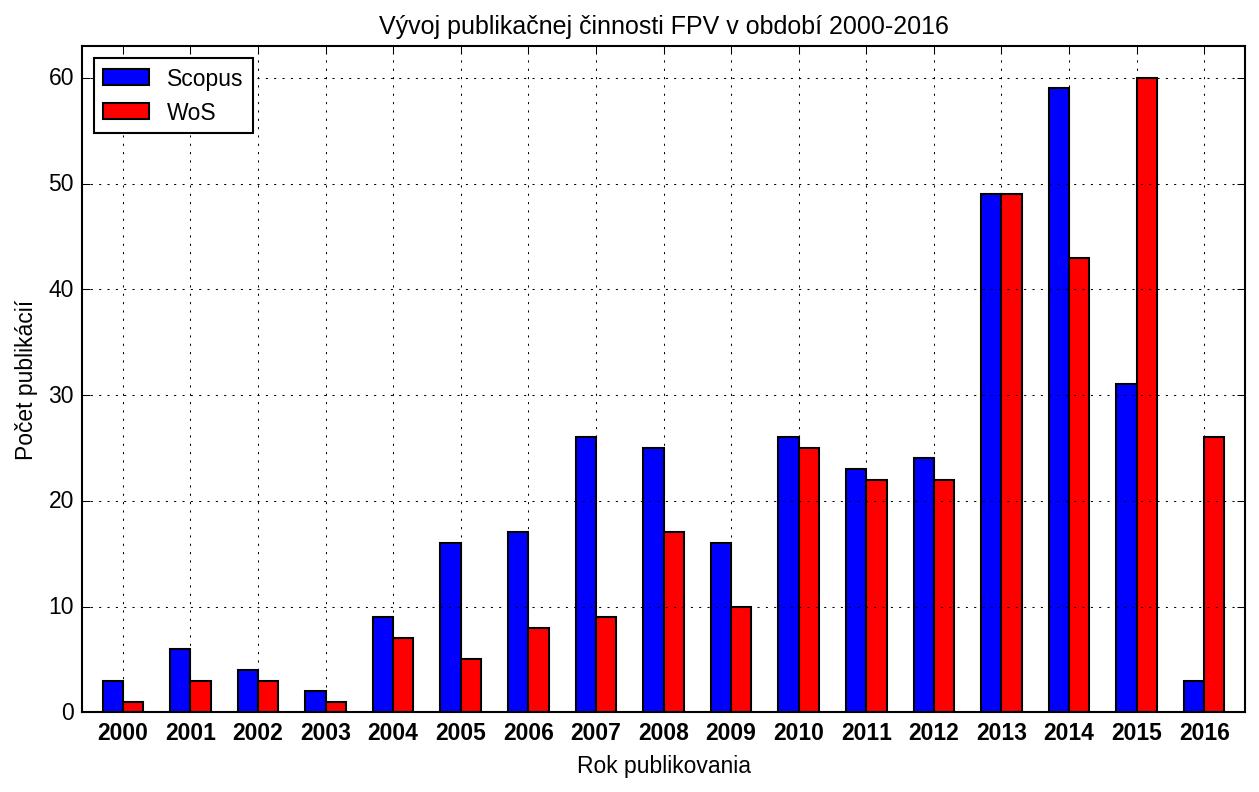
\includegraphics[width=\textwidth]{plot-all-publications-data.png}
  \caption{Vývoj publikačnej činnosti pracovníkov FPV v~období 2000--2016.}
  \label{fig:all.publications.plot}
\end{figure}

Graf na Obrázku~\ref{fig:all.citations.plot} zobrazuje celkový počet citácií
článkov publikovaných v~danom roku.  Rozdiel v~citáciách medzi dátami z~Scopusu
a WoS sú viditeľné hlavne už spomínanom období 2004--2010.  Extrémny rozdiel
citácií na publikácie z~roku 2005 je spôsobený, že v~citačnom registri Scopus je
obsiahnutých 16 článkov z~roku 2005, ktorých 15 sú dobre citované.  WoS obsahuje
iba dva články z~tohto roku: ten necitovaný zo Scopusu a publikáciu, ktorá je
obsiahnutá iba v~databáze z~WoS, ale tiež bez citácií. V~roku 2015 vidíme
dvojnásobný nárast počtu citácií vo WoS oproti Scopusu.  Toto je spôsobené
nárastom publikovania do časopisov, ktoré sú indexované vo WoS ako následok na
tlak na získanie akreditácie.

\begin{figure}
  \centering
  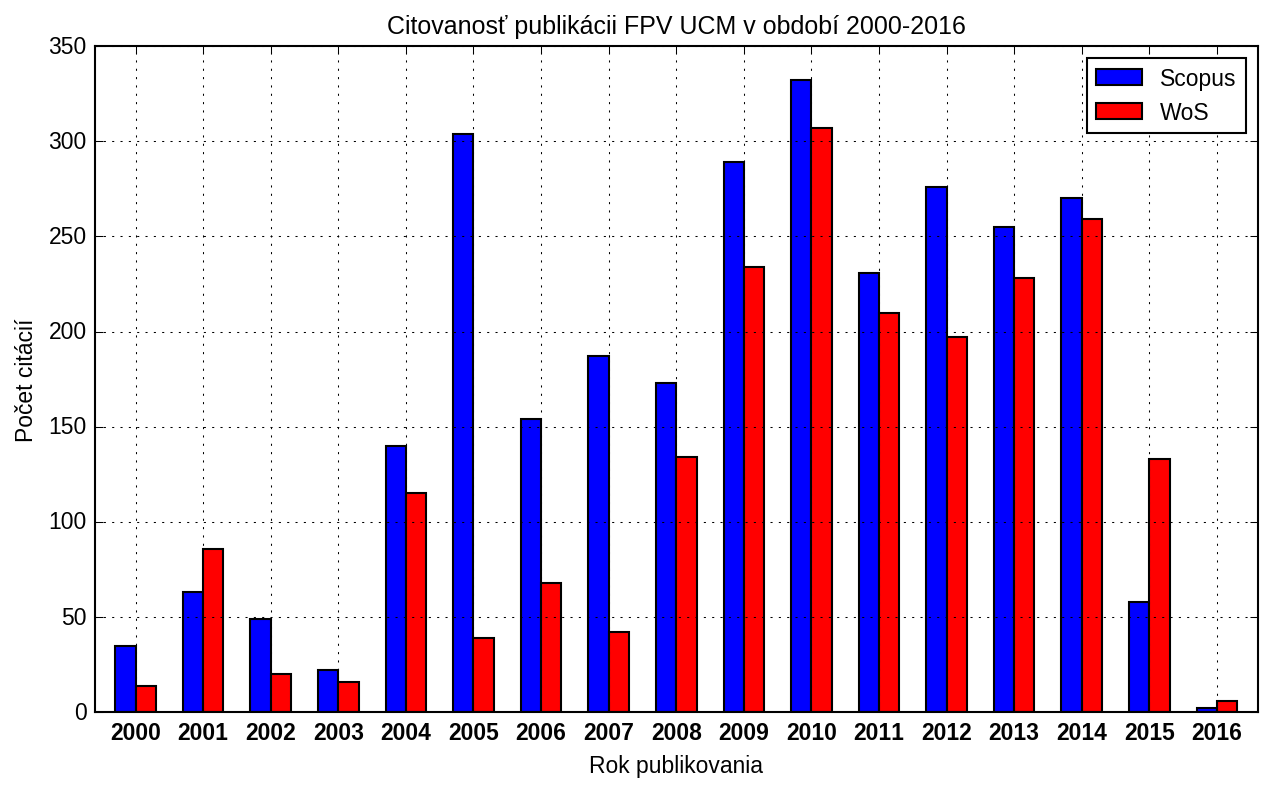
\includegraphics[width=\textwidth]{plot-all-citations-data.png}
  \caption{Citovanosť článkov všetkých pracovníkov FPV za obdobie 2000--2016.}
  \label{fig:all.citations.plot}
\end{figure}


\section{Scientometrické hodnotenie katedier FPV}

Hlavnou časťou tejto práce bola scientometrická analýza jednotlivých katedier
podľa \citet{Kazakis2014a} a \citet{Kazakis2014b,Kazakis2015}. Metodika zahrňuje
výpočet citačných indikátorov zvlášť pre každého vedeckého pracovníka z~danej
inštitúcie. Indikátorom pre katedru predstavuje priemer a medián hodnôt
citačných indikátorov zamestnancov katedry.  Distribúcia indikátorov skupiny
pracovníkov nie je normálna (tzv. gausovská), a~ani sa neblíži
k~normálnej. Z~toho dôvodu si myslíme, že na túto analýzuje je vhodnejšie použiť
medián než aritmetický priemer.

V~Tabuľkách \ref{tab:1-staff.results}, \ref{tab:2-staff.results},
\ref{tab:3-staff.results}, \ref{tab:4-staff.results}, \ref{tab:5-staff.results}
a \ref{tab:6-staff.results} sú uvedené výsledné hodnoty indikátorov každú
katedru FPV.  Namiesto mien katedier sme použili oficiálne skratky (\emph{viď}
Tabuľka \ref{tab:department.review}).  V~Tabuľke \ref{tab:1-staff.results}
stĺpec $n$ zodpovedá počtu vedeckých zamestancov, ktorí boli zahrnutí
do~dátového súboru.  V~stĺpcoch $P$ a $c$ uvádzame sumu všetkých článkov
(Obrázok \ref{fig:publications.plot}) a citácií (Obrázok
\ref{fig:citations.plot}) v~dátom súbore.  Tieto informácie uvádzame pre
ilustráciu, pretože Veľkosti dátových súborov, z~ktorých dane indikátory boli
počítané, určujú presnosť štatistiky. Všetky grafy neobsahujú výsledné hodnoty
Katedry odbornej jazykovej prípravy, pretože boli príliš nízke, z~dôvodu
nedostatku dát.

% Katedra oficiálné skratky katedier\,--\,KB: Katedra biológie; KBt: Katedra biotechnológií; KCh: Katedra chémie; KER: Katedra ekochémie a rádiobiológie; KBf: Katedra biofyziky; KAIM: Katedra aplikovanej informatiky a matematiky; Katedra odbornej jazykovej prípravy. \\
% počet vedeckých pracovníkov danej katedry }

\begin{table}
  \centering\small
  \caption[Hodnotenie FPV\,--\,počet publikácií na autora]%
  {Scientometrické hodnotenie katedier FPV UCM v~Trnave\,--\,počet publikácií na
    autora.}
  \label{tab:1-staff.results}
  \begin{tabularx}{\textwidth}{lXc@{\hspace{2.5em}}c@{\hspace{2.5em}}c@{\hspace{3.5em}}cccc}
    \toprule\noalign{\vspace{.3ex}}
    & & & & & \multicolumn{4}{c}{Počet publikácií na autora} \\
    \cmidrule{6-9}
    Katedra & Cit. register & $n$ & $P$ & $c$ & $\bar{x}$ & $\sigma$ & $\tilde{x}$ & MAD \\[0.3ex]
    \midrule\noalign{\vspace{.5ex}}
    KB   & Scopus & 14 & 380  & 5234  & 9,09  & 13,20 & 3,42  & 3,02 \\
         & WoS    & 13 & 392  & 4982  & 10,66 & 14,44 & 7,20  & 5,18 \\
         & GS     & 14 & 594  & 7289  & 16,88 & 20,77 & 8,92  & 7,42 \\[3ex]
    KBt  & Scopus & 11 & 356  & 11492 & 8,34  & 12,16 & 4,44  & 2,49 \\
         & WoS    & 11 & 351  & 3707  & 7,83  & 10,48 & 5,20  & 3,49 \\
         & GS     & 11 & 828  & 14901 & 23,15 & 24,90 & 12,10 & 5,60 \\[3ex]
    KCh  & Scopus & 18 & 1106 & 19248 & 15,42 & 21,10 & 5,34  & 4,32 \\
         & WoS    & 18 & 1120 & 19223 & 16,14 & 21,85 & 5,76  & 4,54 \\
         & GS     & 18 & 1525 & 25208 & 25,74 & 35,37 & 8,27  & 6,23 \\[3ex]
    KER  & Scopus & 7  & 265  & 1773  & 5,43  & 0,83  & 5,53  & 0,67 \\
         & WoS    & 7  & 275  & 1700  & 5,41  & 0,92  & 5,43  & 0,79 \\
         & GS     & 7  & 543  & 2694  & 4,68  & 0,76  & 4,67  & 0,64 \\[3ex]
    KBf  & Scopus & 5  & 211  & 5232  & 11,85 & 10,71 & 13,85 & 8,50 \\
         & WoS    & 5  & 261  & 6011  & 17,78 & 12,74 & 20,85 & 6,81 \\
         & GS     & 5  & 320  & 8510  & 19,59 & 15,42 & 16,51 & 6,48 \\[3ex]
    KAIM & Scopus & 11 & 91   & 615   & 10,60 & 16,71 & 3,92  & 2,14 \\
         & WoS    & 13 & 106  & 1382  & 10,18 & 19,29 & 2,00  & 0,97 \\
         & GS     & 15 & 151  & 616   & 19,01 & 34,50 & 5,95  & 3,03 \\[3ex]
    KOJP & Scopus & 2  & 3    & 0     & 0,58  & 0,35  & 0,58  & 1,50 \\
         & WoS    & 2  & 2    & 0     & 0,33  & 0,00  & 0,33  & 1,00 \\
         & GS     & 2  & 6    & 3     & 2,00  & 1,88  & 2,00  & 1,33 \\[0.5ex]
    \bottomrule
  \end{tabularx}
\end{table}

Nasleduje artimetický priemer a medián počtu dokumentov na autora (graf
porovnania mediánov je na Obrázku \ref{fig:p/a.plot}).  Pre ilustráciu sme
k~hodnotám artimetického priemeru uviedli štandardné odchýlky.  Na mnohých
prípadoch (najmä pre hodnoty indikátorov: dokumenty na autora a citácie na
dokument) je smerodajná odchýlka vyšia než samotný priemer. Čo indikuje
nedôverihodnosť použitia artimetického priemeru na tento účel. Napriek tomu
v~literatúre sme sa stretli s~častejším použitím aritmetického priemeru než
mediánu \citep{Lazaridis2010}.

Podobne ako u~priemerov, k~mediánu sme vypočítali obdobu smerodanej odchylky
tzv.\,MAD\footnote{Absolútna odchýlka mediánu (ang.\,\emph{Median Absolute
    Deviation}) je robustná štatistická metóda na zistenie rozptylu dát.
  $\mathrm{MAD} = \mathrm{Med}(|X_i - \tilde{X}|)$.  Keďže MAD využíva medián,
  je menej náchylný na extrémne vybočujúce hodnoty, a preto sa používa v~
  distribúciách, ktoré sa príliš odchyľujú od normálnej
  distribúcie.\\\url{http://www.statisticshowto.com/median-absolute-deviation/}}
Rozdiel medzi absolútnou hodnotou mediánu a MAD je nižší než medzi absolútnou
hodnotou priemeru a štandardnej odchýlky znamená, že medián je lepší
ukazovateľom.

\begin{table}
  \centering\small
  \caption[Hodnotenie FPV\,--\,počet citácií na publikáciu a $e$-index]%
  {Scientometrické hodnotenie katedier FPV UCM v~Trnave\,--\,počet citácií na
    publikáciu a $e$-index.}
  \label{tab:2-staff.results}
  \begin{tabularx}{\textwidth}{XXcccc@{\hspace{3ex}}cccc}
    \toprule\noalign{\vspace{.3ex}}
    & & \multicolumn{4}{c}{Počet citácií na publikáciu} & \multicolumn{4}{c}{$e$-index} \\
    \cmidrule{3-6}\cmidrule{7-10}
    Katedra  & Cit. register & $\bar{x}$ & $\sigma$  & $\tilde{x}$ & MAD & $\bar{x}$ & $\sigma$ & $\tilde{x}$  & MAD \\[0.3ex]
    \midrule\noalign{\vspace{.5ex}}
    KB   & Scopus & 7,74  & 7,75  & 5,88  & 3,99  & 9,03  & 9,53  & 7,49  & 4,06  \\
         & WoS    & 7,77  & 7,16  & 6,17  & 3,77  & 9,14  & 9,36  & 7,75  & 5,10  \\
         & GS     & 17,88 & 7,40  & 6,50  & 3,31  & 26,88 & 11,45 & 9,83  & 3,95  \\[3ex]
    KBt  & Scopus & 13,54 & 18,36 & 7,76  & 5,29  & 16,12 & 24,59 & 9,27  & 1,92  \\
         & WoS    & 7,40  & 5,74  & 5,70  & 4,70  & 9,63  & 7,62  & 9,00  & 2,45  \\
         & GS     & 9,93  & 14,14 & 4,27  & 3,33  & 18,96 & 26,42 & 12,45 & 2,20  \\[3ex]
    KCh  & Scopus & 12,45 & 12,03 & 10,97 & 1,92  & 14,70 & 16,23 & 10,82 & 4,42  \\
         & WoS    & 12,62 & 10,91 & 11,81 & 2,98  & 14,94 & 15,74 & 11,86 & 4,52  \\
         & GS     & 11,35 & 10,87 & 10,35 & 3,30  & 17,21 & 18,65 & 13,25 & 6,12  \\[3ex]
    KER  & Scopus & 5,49  & 2,73  & 6,63  & 1,19  & 7,63  & 3,84  & 9,27  & 0,27  \\
         & WoS    & 5,21  & 2,28  & 6,06  & 0,92  & 7,26  & 4,46  & 8,31  & 0,75  \\
         & GS     & 4,53  & 1,80  & 4,93  & 0,82  & 9,60  & 4,64  & 11,96 & 0,53  \\[3ex]
    KBf  & Scopus & 16,58 & 13,35 & 13,34 & 13,34 & 19,52 & 16,86 & 18,65 & 16,45 \\
         & WoS    & 16,44 & 15,49 & 14,68 & 9,73  & 23,99 & 19,66 & 25,16 & 14,00 \\
         & GS     & 18,44 & 15,93 & 15,90 & 14,42 & 25,31 & 23,36 & 21,70 & 21,70 \\[3ex]
    KAIM & Scopus & 3,57  & 5,24  & 0,80  & 0,80  & 5,28  & 7,80  & 1,00  & 1,00  \\
         & WoS    & 3,16  & 5,53  & 0,25  & 0,25  & 4,83  & 9,37  & 0,00  & 0,00  \\
         & GS     & 2,83  & 3,58  & 1,00  & 1,00  & 6,25  & 8,57  & 2,00  & 2,00  \\[3ex]
    KOJP & Scopus & --    & --    & --    & --    & --    & --    & --    & --    \\
         & WoS    & --    & --    & --    & --    & --    & --    & --    & --    \\
         & GS     & 0,50  & 0,00  & 0,25  & 0,25  & 0,50  & 0,71  & 0,50  & 0,50  \\[0.5ex]
    \bottomrule
  \end{tabularx}
\end{table}

Tabuľka \ref{tab:2-staff.results} obsahuje počet citácií na dokument (grafické
porovnanie mediánov v~grafe Obrázok \ref{fig:c/p.plot}) a Zhangov $e$-index.
Hodnoty dát Katedry odbornej jazykovej prípravy zo Scopusu a WoS nepočítali,
pretože neboli vôbec citované.  štandardných odchýlok a hodnoty aritmetických
priemerov indikátorov počtu publikácií na autora a počtu citácií na dokument
(Tabuľky \ref{tab:1-staff.results} a \ref{tab:1-staff.results}), spozorujeme, že
v~mnohých prípadoch hodnota štandardnej odchýlky presahuje hodnotu priemeru.  Čo
znamená, že základné indikátory ako počet publikácií na~autora a počet citácií
na dokument nie sú vhodné na scientometrickú analýzu tohoto typu.  Zhangov
$e$-index je modifikácia $h$-indexu, ktorá je citlivá na veľmi citované články
v~malom súbore publikácií (\emph{viď} pokapitola \ref{sec:e-index}).  Na základe
výsledkov Katedry biofyziky (Tabuľka \ref{tab:2-staff.results}) môžeme názorne
vidieť, že mediány $e$-indexu sú rádovo väčšie od ostatných (graficky
znáznornené na Obrázku \ref{fig:e-index.plot}).

Hodnoty citačných indikátorov $h$-index a $g$-index sú uvedené v~tabuľke
\ref{tab:3-staff.results} a mediány sú graficky znázornené na Obrázkoch
\ref{fig:h-index.plot} a \ref{fig:g-index.plot}.  Rozdiel medzi hodnotami
priemeru a mediánu Katedry aplikovanej informatiky a je spôsobený výskytom
niekoľko veľmi citovaných pracovníkov oproti ostatným, ktorí sú minimálne
citovaní.

\citet{Kazakis2015} scientometricky porovnával katedry chemického inžinierstva
troch gréckych univerzít (Atény, Solún a Patra).  V~Tabuľke
\ref{tab:kazakis.results} sme porovnali naše výsledky s~Kazakisovymi. Napriek
tomu, že Gréci čerpali iba z~citačného registru Scopus, my sme porovnali
indikátory zo všetkých použitých citačných registrov. Na prvý pohľad si všimneme
rozdiel v~počte pracovníkov (v~tabuľke označené ako $n$).  Grécke katedry
zahrňujú ďaleko viacej ľudí (katedra v~Aténach dokonca až 72 akademikov) než
Katedra chémie s~18 pracovníkmi.  Hodnoty priemerného $h$-index a $g$-indexu
Katedry chémie sú zhruba o~tretinu nižšie než gréckych katedier.  Veľký rozdiel
predstavujú príliš vysoké štandardné odchýlky (ktoré skoro dosahujú hodnotu
priemeru). Pre porovnanie Gréci majú menšie štantardné odchýlky.  Myslíme si, že
lepší indikátorom sú mediány, pretože MAD hodnoty sú nižšie než smerodajné
odchýlky.  V~tomto prípade sú mediány $h$-index a $g$-indexu Katedry chémie
približne 100\,\% nižšie než gréckych katedier. , že Katedra chémie má približne
dvakrát menej zamestnancov, tak je výsledok očakávateľný.

\citet{Lazaridis2010} vypočítal priemerný $h$-index gréckych chemických katedier
prestížnych gréckych univerzít (Krétska, Patraska, Solúnska, Ioanninanska, a
Aténska).  Dáta čerpal z~citačného registru WoS, pričom na výpočet $h$-index
používal webové rozhranie WoS, alebo ho počítal ručne.  V~Tabuľke
\ref{tab:lazaridis.results} sú porovnané priemerné $h$-index katedier spomenutých
gréckych univerzít a naše výsledky pre Katedru chémie. Síce priemerný $h$-index
gréckych katedier je porovnateľný s~KCh (s~výnimkou Krétskej univerzity), ale
dátový súbor je výrazne menší. Zdá sa nám nepravdepodobné aby taká inštitúcia
mala také male množstvo publikácií.  Autor o~získavaní dát píše iba o~problémoch
s~gréckymi menami v~anglickej databáze WoS. V~neposlednom rade nesmieme zabúdať,
že autor neuvádza smerodajnú odchýlku a je nám dobre známe, že distribúcia
citačných indikátorov nemusí byť podobná normálnemu rozdeleniu. V~prípade
distribúcie, ktorá sa príliš líši od normálnej distribúcie, sa použitie
aritmetického priemeru stáva nevhodným.

Na grafickom porovaní mediánov $h$-indexu (\emph{viď} podkapitola
\ref{sec:h-index}) a $g$-indexu (\emph{viď} podkapitola \ref{sec:g-index}
katedier FPV môžeme vidieť vyrazný rozdiel medzi Katedrou biofyziky a ostatnými
katedrami, najmä Katedry chémie, ktorá výrazne zaostáva za KBf napriek
najvyšiemu počtu publikácií a citácií (\emph{viď} Obrázky
\ref{fig:publications.plot} a \ref{fig:citations.plot}).  Tento trend je možné
pozorovať na každom hodnotení FPV pomocou citačných indikátorov (Obrázky
\ref{fig:p/a.plot}, \ref{fig:c/p.plot}, \ref{fig:h-index.plot},
\ref{fig:g-index.plot}, \ref{fig:e-index.plot}, \ref{fig:hc-index.plot},
\ref{fig:hi-index.plot}, \ref{fig:hinorm.plot}, \ref{fig:hm-index.plot},
\ref{fig:awcr.plot}, \ref{fig:aw-index.plot}).

Tabuľka \ref{tab:4-staff.results} ukazuje výsledné hodnoty individuálneho
$h$-indexu ($h_{\mathrm{I}}$-index, \emph{viď} podkapitola \ref{sec:hi-index}) a
jeho variante pre program Publish or Perish (\emph{viď} podkapitola
\ref{sec:pop}) $h_{\mathrm{I,norm}}$ (\emph{viď} podkapitola
\ref{sec:hinorm}). Tieto indikátory normujú $h$-index na počet
spoluautorov. Rádovo vyšie hodnoty aritmetického priemeru oboch indikátorov GS
je pravdepodobne spôsobený vlastnosťou Google Scholaru: automaticky zoznam
autorov zužuje na 3-5 položiek (\emph{viď} podkapitola \ref{sec:gs}), čím umelo
zvyšuje hodnotu $h_{\mathrm{I}}$-index a $h_{\mathrm{I,norm}}$.  Rozdiel
mediánov jednotlivých katedier je graficky zobrazený na Obrázkoch
\ref{fig:hi-index.plot} a \ref{fig:hinorm.plot}.

V~Tabuľke \ref{tab:5-staff.results} uvádzame prehľad výsledkov citačnej
frekvencie váhovanej podľa veku (AWCR) a $AW$-index (\emph{viď} podkapitola
\ref{sec:aw-index}). Ako názov napovedá tieto indikátory znižujú váhu starších
publikácií. Využíva sa hlavne na porovnávanie vedcov s~rôznymi akademickým
vekom, pretože starší profesor s~bohatou akademickou kariérov, ale na dôchodku
sa javý produktívnejší v~očiach $h$-indexu ako mladý vedec na začiatku kariéry
v~plnej sile. Priemerné hodoty AWCR podliehajú veľkej chybe, preto sme na graf
použili mediány (Obrázky \ref{fig:awcr.plot} a \ref{fig:aw-index.plot}).

Na tabuľke \ref{tab:6-staff.results} sú zobrazené výsledné hodnoty súčasného
$h$-indexu ($h^{\mathrm{c}}$-index) a multiautorského $h$-indexu
($h_{\mathrm{m}}$-index).  Súčasný $h$-index je ďalší indikátor, ktorý zahrnuje
starnutie článkov (\emph{viď} podkapitola \ref{sec:hc-index}) a multiautorský
$h$-index znižuje hodnotu, podľa počtu autorov (vid. podkapitola
\ref{sec:hm-index}).  Mediány týchto citačných indikátorov pre FPV sú vykreslené
na Obrázku \ref{fig:hc-index.plot} a Obrázku \ref{fig:hm-index.plot}.

\begin{SCtable}
\centering\small
  \caption[Porovnanie KCh FPV a kat. chem. inžinierstva  troch gréckych univerzít]%
  {Porovnanie citačných indikátorov Katedry chémie FPV a katedier chemického
    inžinierstva troch gréckych univerzít \citep{Kazakis2015}}
  \label{tab:kazakis.results}
  \begin{tabular}{lcccccc}
    \toprule\noalign{\vspace{.3ex}}
    & \multicolumn{3}{c}{Katedra chémie FPV} & \multicolumn{3}{c}{\citet{Kazakis2015}}  \\
    Indikátor & Scopus & WoS   & GS    &  Atény     & Solún      & Patra      \\[0.3ex]
    \midrule\noalign{\vspace{.5ex}}
    $n$         & 18     & 18    & 18    & 72    & 34    & 30    \\
    $P$         & 1106   & 1120  & 1525  & 4463  & 2253  & 2573  \\
    P/A$^\dagger$         & 15,42  & 16,14 & 25,74 & 62    & 66,3  & 85,8  \\
    $c$         & 19248  & 19223 & 25208 & 74368 & 39695 & 63718 \\
    C/P$^\ddagger$         & 12,45  & 12,62 & 11,35 & 16,7  & 17,6  & 24,8  \\[1ex]
    $\bar{h}$   & 11,78  & 11,94 & 13,61 & 16,3  & 16,8  & 21,3  \\
    $\sigma (h)$ & 11,70  & 11,70 & 12,99 & 8     & 8,5   & 1,5   \\
    $\tilde{h}$ & 7,50   & 7,50  & 9,00  & 15,5  & 17    & 18    \\
    $\bar{g}$   & 19,83  & 20,22 & 23,56 & 26,8  & 28,3  & 35,5  \\
    $\sigma (g)$  & 22,23  & 21,68 & 24,89 & 12,6  & 13,9  & 23    \\
    $\tilde{g}$  & 14,50  & 15,00 & 16,50 & 26,5  & 27    & 30,5  \\[0.5ex]
    \bottomrule
    \multicolumn{7}{l}{\footnotesize $^\dagger$ počet autorov na publikáciu; $^\ddagger$ počet citácii na publikáciu} \\
  \end{tabular}
\end{SCtable}

\begin{table}
  \centering\small
  \caption[Porovnanie KCh FPV a chemických katedier vybraných gréckych univerzít]%
  {Porovnanie citačných indikátorov Katedry chémie FPV  a katedier chémie
    piatich gréckych univerzít \citep{Lazaridis2010}}
  \label{tab:lazaridis.results}
  \begin{tabularx}{\textwidth}{Xccclccccc}
    \toprule\noalign{\vspace{.5ex}}
    & \multicolumn{3}{c}{Katedra chémie FPV}& \phantom{M} & \multicolumn{5}{c}{\citet{Lazaridis2010}} \\
    Indikátor  & Scopus & WoS   & GS                 &  & Kréta & Patra & Solún & Ioaninna & Atény \\[0.3ex]
    \midrule\noalign{\vspace{.5ex}}
    $P$         & 1106   & 1120  & 1525               & & 56    & 61    & 41    & 48       & 219   \\
    $\bar{h}$  & 11,78  & 11,94 & 13,61              & & 16,6  & 12,6  & 10,4  & 10,3     & 9,0   \\[0.5ex]
    \bottomrule
  \end{tabularx}
\end{table}

\begin{table}
  \centering\small
  \caption[Porovnanie KEB, KBt a vybranej skupiny enviromentalistov]%
  {Porovnanie citačných indikátorov Katedry ekochémie a rádiobiológie a vybranej
    skupiny vedcov z~oblasti enviromentalistiky, ktorí sa zúčastnili projektu
    ACUMEN FP7 \citep{Wildgaard2015}.}
  \label{tab:wildgaard.results}
  \begin{tabularx}{\textwidth}{Xlcccccccccc}
    \toprule\noalign{\vspace{.3ex}}
    kat. &Cit.\,reg. & $n$ & $p$ & $c$ & A/P$^\dagger$ & C/P$^\ddagger$ & AWCR & AW & $h$ & $g$ & $e$ \\[0.3ex]
    \midrule\noalign{\vspace{.5ex}}
    ENV & WoS & 99 & 3228 & 34851 & 3,1   & 7,8   & 42,4  & 5,4  & 8,5  & 13,1  & 9,1   \\
        & GS  & 99 & 7425 & 62351 & 3,2   & 7,6   & 76,1  & 7,5  & 11,9 & 18,4  & 13,2  \\[2ex]
    KER & WoS & 7  & 275  & 1700  & 5,41  & 5,21  & 40,24 & 5,82 & 7,57 & 11    & 7,26  \\
        & GS  & 7  & 543  & 2694  & 4,68  & 4,53  & 74,13 & 8,04 & 9,43 & 14,71 & 9,6   \\[2ex]
    KBt & WoS & 1  & 351  & 3707  & 7,83  & 7,4   & 33,76 & 4,71 & 6,55 & 12,09 & 9,63  \\
        & GS  & 1  & 828  & 14901 & 23,15 & 14,14 & 84,97 & 7,48 & 9,73 & 22,55 & 18,96 \\[0.5ex]
    \bottomrule

    \multicolumn{12}{l}{\footnotesize $^\dagger$ počet autorov na publikáciu; $^\ddagger$ počet citácii na publikáciu} \\
  \end{tabularx}
\end{table}

\citet{Wildgaard2015} porovnával 17 citačných indikátorov na vzorke vedcov
z~rôznych vedných oblastí. Jednou z~nich bola enviromentalistika. Vzorka
obsahovala $n$ akademikov od doktorov po profesorov. Porovnávali sme Katedru
ekochémie a rádiobiológie (KER), Katedru biotechnlógií a už vyšie uvedenú vzorku
vedcov.  Porovnanie hodnôt citačných indikátorov je uvedené v~Tabuľke
\ref{tab:wildgaard.results}.  Dáta boli získané z~citačných registrov \emph{Web
  of Science} (WoS) a \emph{Google Scholar} (GS).  Napriek veľkému rozdielu
v~počte akademikov ($n$), vo väčšine prípadov katedry FPV vykazujú väčšie
kvality než skupina enviromentalistov. Ale treba brať do úvahy, že skupina nie
je viazana afiliáciou, ale účasťou na projekte ACUMEN
FP7\footnote{\url{http://research-acumen.eu/}}.

Vytvorili sme zoznam časopisov s~najväčším počtom $n$ publikácií (zoradené
zostupne) z~citačných registrov WoS a Scopus (\emph{viď} Príloha).  Tabuľka
zahrňuje najpoužívanejšie citačné indikátory na hodnotenie časopisov: impakt
faktor (IF); Scimago rang časopisov; SciteCore a SNIP (\emph{viď} Tabuľka
\ref{tab:indicators.review}).

Zo scientometrického hodnotenia vyplýva, že najproduktívnejšia katedra je
Katedra biofyziky, pretože dosahuje najvyšie hodnoty mediánov citačných
indikátorov napriek výraznému rozdielu v~absolútnych hodnotách počtu publikácií
a citácií oproti Katedre chémie. Síce najhoršie sa umiestnila Katedra odbornej
jazykovej prípravy (KOJP). Ako už názov napovedá táto katedra sa zameriava na
prírodné vedy. Podarilo sa nám vyhľadať do desať publikácií s~minimom citácií.
Preto sme ich dáta nevykresľovali do grafov.

Ďalšia katedra je katedra aplikovanej informatiky a matematiky (KAIM) má na
internetových stránkach uvedený relatívne rozsiahly zoznam pracovníkov (15), ale
publikácie všetkých uvedených pracovníkov sa nám podarilo vyhľadať iba
z~citačného registru Google Scholar (GS), ktorý prehľadáva všetky voľne
prístupné publikácie. Teda má prístup k~najväčšiemu počtu dokumentov. Extrémné
hodnoty smerodajnej dochýlky (napr. v~Tabuľke \ref{tab:5-staff.results}) sú
spôsobené nevyváženou distribúciou citácií, teda valnej väčšine citácií katedry
prislúcha niekoľkým veľmi citovaných pracovníkom. Ostatní nemajú takmer žiadne
citácie.

Katedra biológie, biotechnológií, ekochémie a rádiobiológie a dokonca aj chémie
sú zhruba na rovnakej úrovni. Pri niektorých indikátoroch vyniká jedna, či
druhá, ale s~celkovým hodnotením a započítaním chyby nie je možné ďalej určiť
poradie.

\begin{figure}
  \centering
  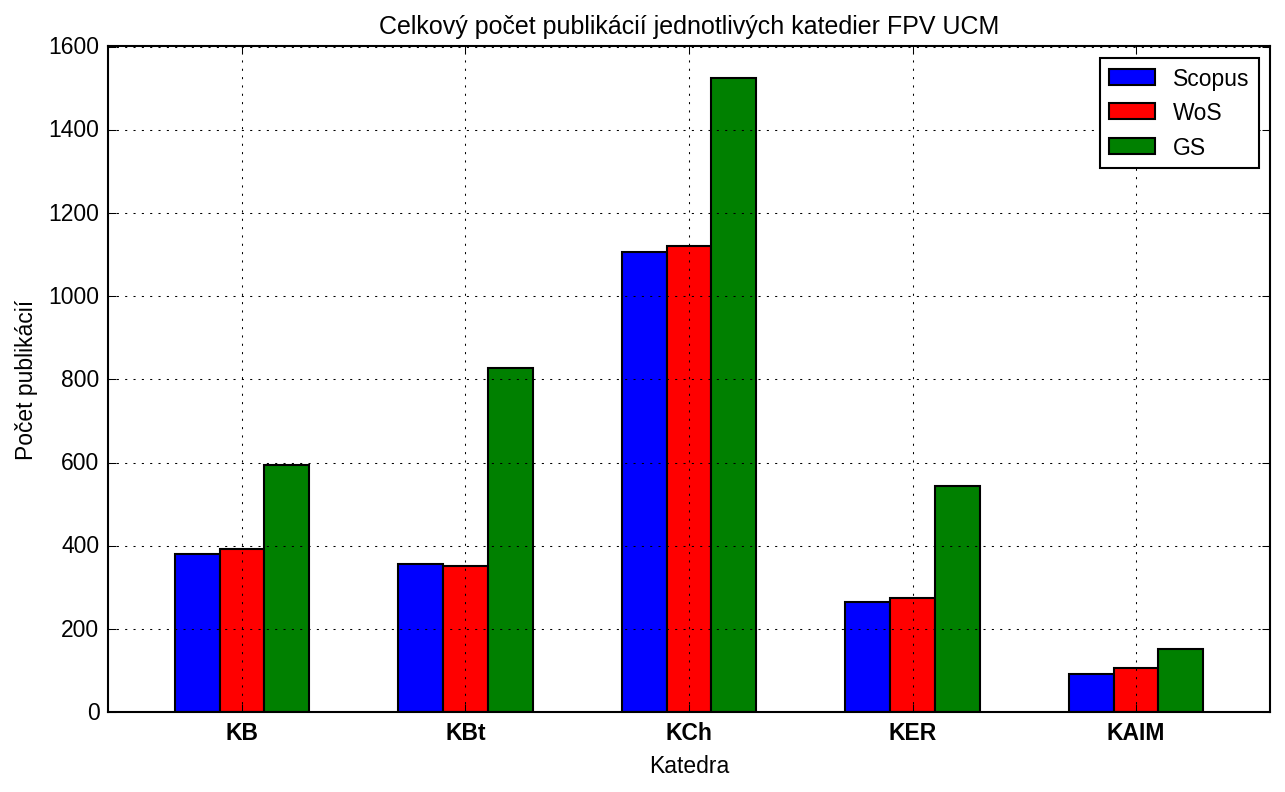
\includegraphics[width=\textwidth]{plot-results-data-papers.png}
  \caption{Celkový počet publikácií jednotlivých katedier FPV UCM v~Trnave}
  \label{fig:publications.plot}
\end{figure}

\begin{figure}
  \centering
  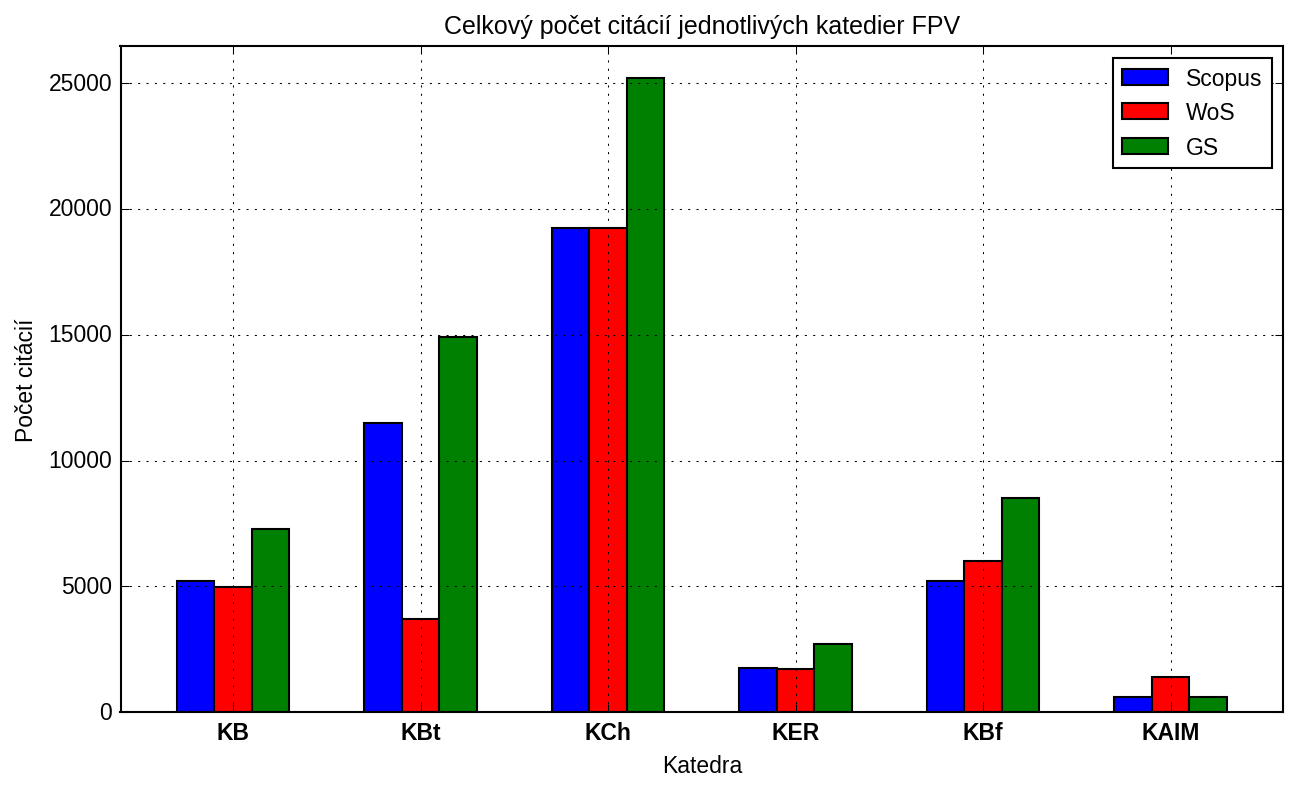
\includegraphics[width=\textwidth]{plot-results-data-citations.png}
  \caption{Celkový počet citácií jednotlivých katedier FPV UCM v~Trnave}
  \label{fig:citations.plot}
\end{figure}

\begin{figure}
  \centering
  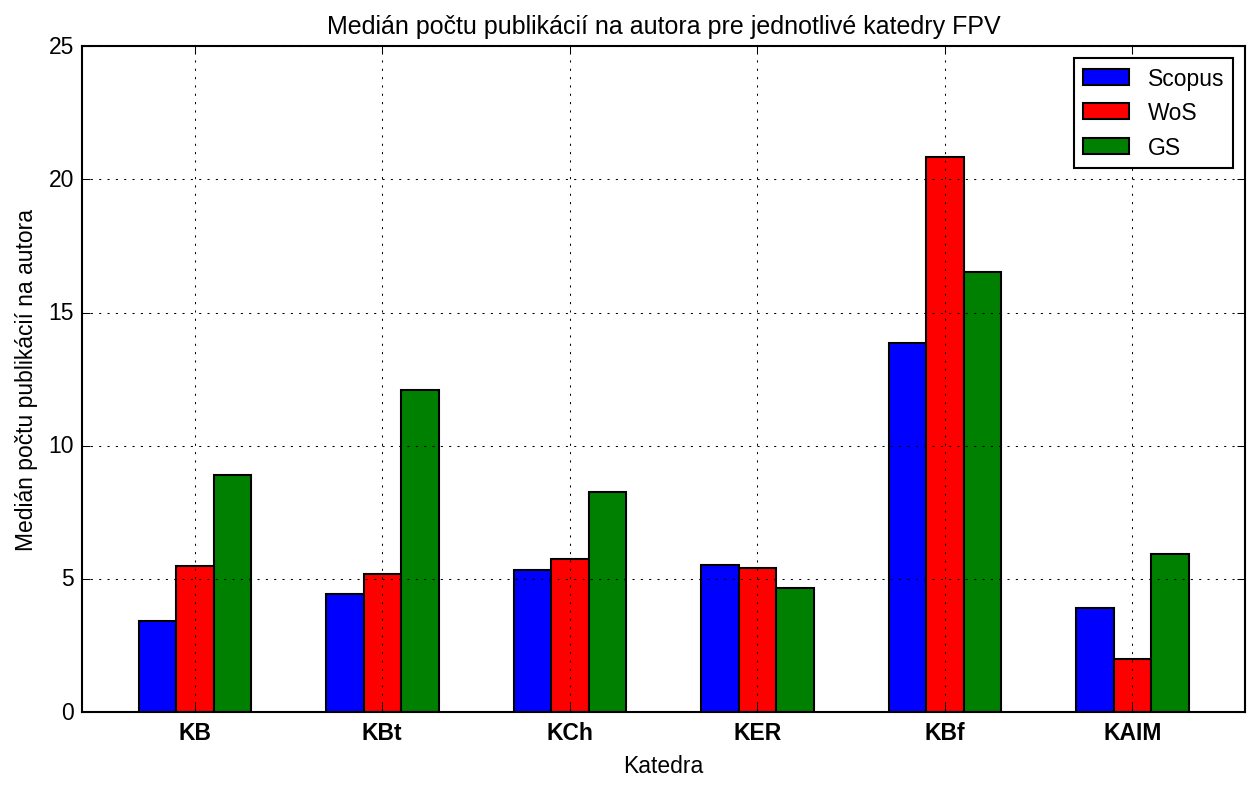
\includegraphics[width=\textwidth]{plot-results-data-papers_author.png}
  \caption{Medián počtu publikácií na autora pre jednotlivé katedry FPV UCM v~Trnave}
  \label{fig:p/a.plot}
\end{figure}


\begin{figure}
  \centering
  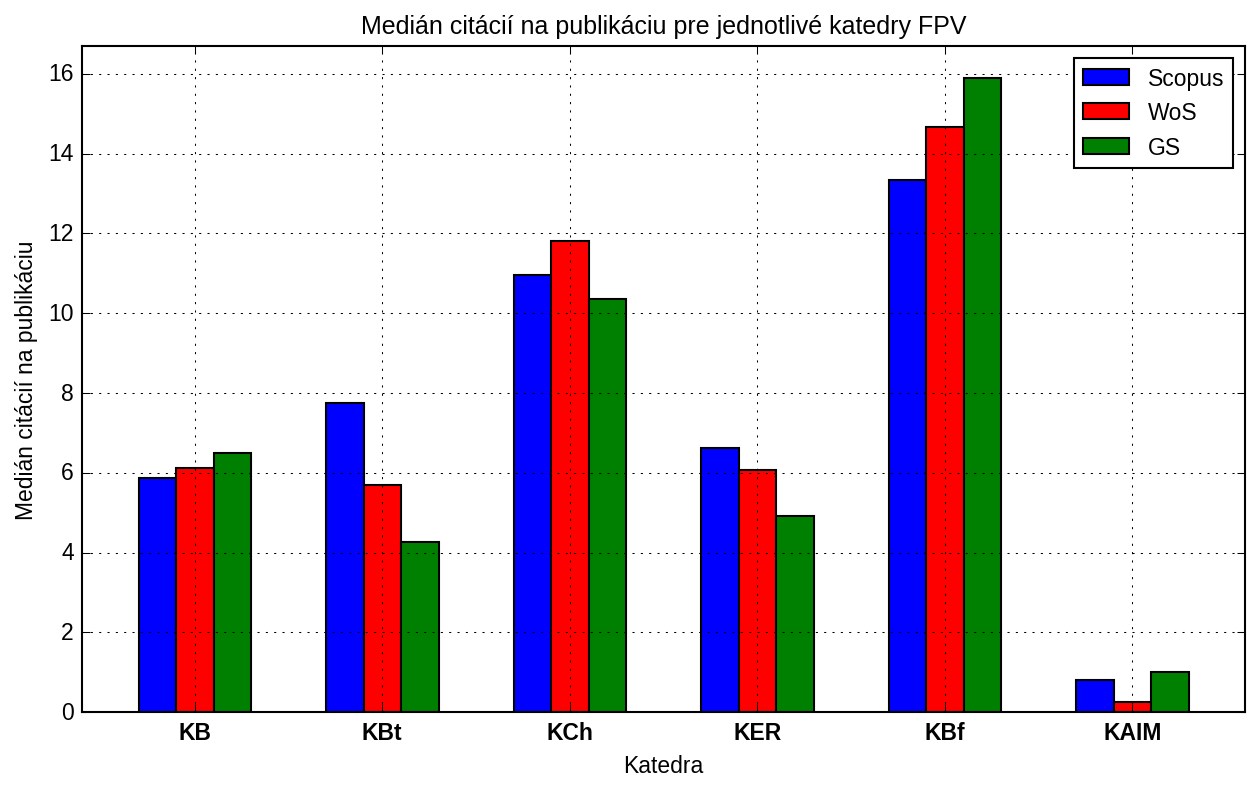
\includegraphics[width=\textwidth]{plot-results-data-cites_paper.png}
  \caption{Medián citácií na publikáciu pre jednotlivé katedry FPV UCM v~Trnave}
  \label{fig:c/p.plot}
\end{figure}

\begin{table}
  \centering\small
  \caption[Hodnotenie FPV\,--\,$h$-index a $g$-index]%
  {Scientometrické hodnotenie katedier FPV UCM v~Trnave\,--\,$h$-index a $g$-index.}
  \label{tab:3-staff.results}
  \begin{tabularx}{\textwidth}{XXcccc@{\hspace{3ex}}cccc}
    \toprule\noalign{\vspace{.3ex}}
    & & \multicolumn{4}{c}{$h$-index} & \multicolumn{4}{c}{$g$-index} \\
    \cmidrule{3-6}\cmidrule{7-10}
    Katedra & Cit. register & $\bar{x}$ & $\sigma$ & $\tilde{x}$ & MAD & $\bar{x}$ & $\sigma$ & $\tilde{x}$ & MAD \\[0.3ex]
    \midrule\noalign{\vspace{.5ex}}
    KB   & Scopus & 7,93  & 7,65  & 6,50  & 4,50  & 12,71 & 13,22 & 11,00 & 7,00  \\
         & WoS    & 8,23  & 7,57  & 7,00  & 5,00  & 12,92 & 13,07 & 10,50 & 7,50  \\
         & GS     & 18,88 & 8,39  & 6,00  & 3,50  & 19,88 & 15,19 & 11,50 & 6,00  \\[3ex]
    KBt  & Scopus & 7,45  & 8,07  & 5,00  & 3,00  & 18,36 & 27,16 & 12,00 & 4,00  \\
         & WoS    & 6,55  & 7,38  & 4,00  & 3,00  & 12,09 & 11,04 & 10,00 & 3,00  \\
         & GS     & 9,73  & 8,83  & 7,00  & 4,00  & 22,55 & 28,96 & 16,00 & 4,00  \\[3ex]
    KCh  & Scopus & 11,78 & 11,70 & 7,50  & 4,50  & 19,83 & 22,23 & 14,50 & 9,50  \\
         & WoS    & 11,94 & 11,70 & 7,50  & 4,50  & 20,22 & 21,68 & 15,00 & 9,50  \\
         & GS     & 13,61 & 12,99 & 9,00  & 5,50  & 23,56 & 24,89 & 16,50 & 9,50  \\[3ex]
    KER  & Scopus & 8,00  & 4,40  & 9,00  & 3,00  & 11,71 & 6,55  & 14,00 & 2,00  \\
         & WoS    & 7,57  & 4,35  & 8,00  & 4,00  & 11,00 & 6,88  & 12,00 & 3,00  \\
         & GS     & 9,43  & 4,76  & 11,00 & 2,00  & 14,71 & 7,11  & 18,00 & 2,00  \\[3ex]
    KBf  & Scopus & 12,80 & 10,57 & 15,00 & 10,00 & 24,80 & 21,61 & 26,00 & 20,00 \\
         & WoS    & 15,50 & 12,37 & 16,00 & 8,00  & 30,75 & 25,00 & 32,00 & 17,50 \\
         & GS     & 16,00 & 13,17 & 17,00 & 13,00 & 31,80 & 28,26 & 30,00 & 23,00 \\[3ex]
    KAIM & Scopus & 3,91  & 5,82  & 1,00  & 1,00  & 6,82  & 10,42 & 1,00  & 1,00  \\
         & WoS    & 3,85  & 7,06  & 1,00  & 1,00  & 6,62  & 12,50 & 1,00  & 1,00  \\
         & GS     & 4,33  & 6,00  & 2,00  & 2,00  & 8,13  & 11,28 & 3,00  & 3,00  \\[3ex]
    KOJP & Scopus & --    & --    & --    & --    & --    & --    & --    & --    \\
         & WoS    & --    & --    & --    & --    & --    & --    & --    & --    \\
         & GS     & 1,00  & 0,00  & 0,50  & 0,50  & 1,00  & 0,00  & 0,50  & 0,50  \\[0.5ex]
    \bottomrule
  \end{tabularx}
\end{table}

\begin{figure}
  \centering
  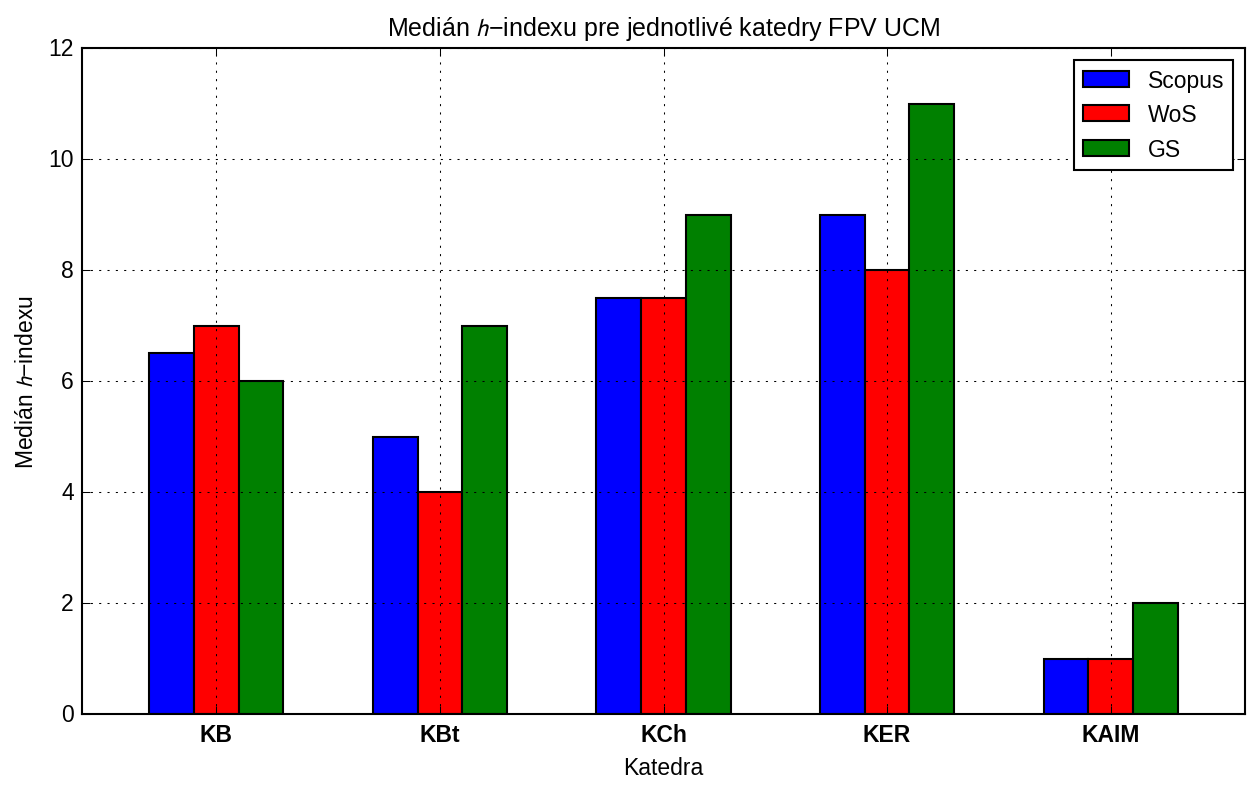
\includegraphics[width=\textwidth]{plot-results-data-h_index.png}
  \caption{Medián $h$-indexu pre jednotlivé katedry FPV UCM v~Trnave}
  \label{fig:h-index.plot}
\end{figure}

\begin{figure}
  \centering
  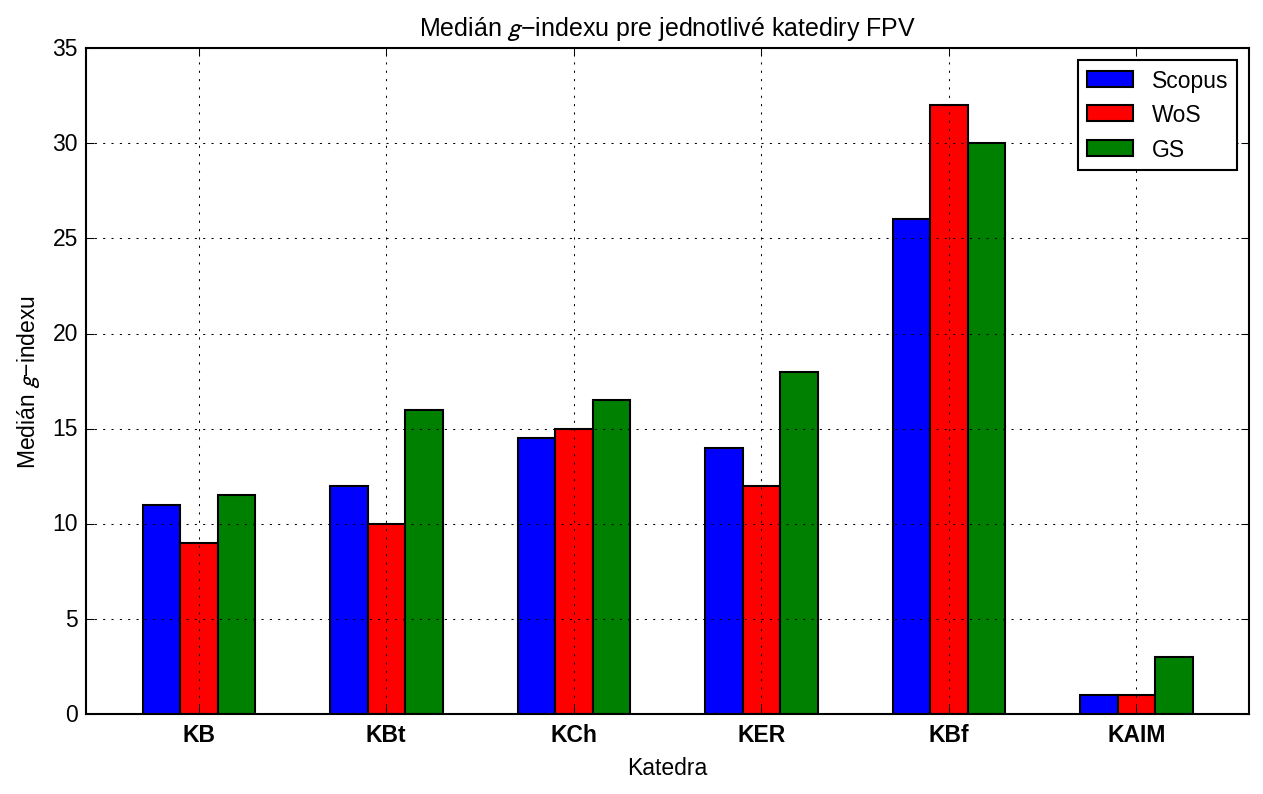
\includegraphics[width=\textwidth]{plot-results-data-g_index.png}
  \caption{Medián $g$-indexu pre jednotlivé katedry FPV UCM v~Trnave}
  \label{fig:g-index.plot}
\end{figure}

\begin{table}
  \centering\small
  \caption[Hodnotenie FPV\,--\,$h_{\mathrm{I}}$-index a $h_{\mathrm{I,norm}}$]%
  {Scientometrické hodnotenie katedier FPV UCM v~Trnave\,--\,$h_{\mathrm{I}}$-index a $h_{\mathrm{I,norm}}$}
  \label{tab:4-staff.results}
  \begin{tabularx}{\textwidth}{XXcccc@{\hspace{3ex}}cccc}
    \toprule\noalign{\vspace{.3ex}}
    & & \multicolumn{4}{c}{$h_{\mathrm{I}}$-index} & \multicolumn{4}{c}{$h_{\mathrm{I,norm}}$} \\
    \cmidrule{3-6}\cmidrule{7-10}
    Katedra & Cit. register& $\bar{x}$ & $\sigma$ & $\tilde{x}$ & MAD & $\bar{x}$ & $\sigma$ & $\tilde{x}$ & MAD \\[0.3ex]
    \midrule\noalign{\vspace{.5ex}}
    KB   & Scopus & 1,94  & 2,82 & 1,10 & 0,85 & 4,00  & 4,96 & 2,50 & 1,50 \\
         & WoS    & 2,08  & 2,88 & 1,46 & 0,89 & 4,23  & 5,40 & 3,00 & 2,00 \\
         & GS     & 21,88 & 3,40 & 1,48 & 0,84 & 22,88 & 5,85 & 3,50 & 2,00 \\[3ex]
    KBt  & Scopus & 1,46  & 1,66 & 0,84 & 0,34 & 3,64  & 2,94 & 3,00 & 0,00 \\
         & WoS    & 1,24  & 1,47 & 0,82 & 0,46 & 3,36  & 2,80 & 3,00 & 1,00 \\
         & GS     & 2,41  & 2,15 & 1,73 & 0,71 & 5,00  & 3,74 & 4,00 & 1,00 \\[3ex]
    KCh  & Scopus & 2,10  & 1,64 & 1,55 & 0,86 & 5,17  & 4,72 & 4,00 & 2,00 \\
         & WoS    & 2,20  & 1,77 & 1,53 & 0,94 & 5,50  & 4,82 & 4,00 & 2,00 \\
         & GS     & 3,02  & 2,87 & 2,08 & 1,23 & 6,61  & 6,55 & 5,00 & 2,50 \\[3ex]
    KER  & Scopus & 1,56  & 0,93 & 1,72 & 0,53 & 3,14  & 1,68 & 3,00 & 2,00 \\
         & WoS    & 1,46  & 0,93 & 1,65 & 0,36 & 3,00  & 2,00 & 3,00 & 1,00 \\
         & GS     & 1,88  & 1,02 & 1,94 & 0,54 & 4,14  & 2,04 & 5,00 & 1,00 \\[3ex]
    KBf  & Scopus & 2,49  & 2,29 & 2,50 & 1,88 & 6,80  & 6,06 & 6,00 & 6,00 \\
         & WoS    & 3,17  & 2,86 & 2,91 & 1,73 & 8,00  & 6,73 & 8,00 & 5,00 \\
         & GS     & 3,44  & 2,90 & 3,04 & 2,04 & 8,60  & 6,84 & 8,00 & 6,00 \\[3ex]
    KAIM & Scopus & 1,74  & 2,52 & 0,50 & 0,50 & 2,73  & 3,69 & 1,00 & 1,00 \\
         & WoS    & 1,60  & 2,75 & 0,50 & 0,50 & 2,46  & 4,35 & 1,00 & 1,00 \\
         & GS     & 1,66  & 2,28 & 1,00 & 0,67 & 2,93  & 4,17 & 1,00 & 1,00 \\[3ex]
    KOJP & Scopus & --    & --   & --   & --   & --    & --   & --   & --   \\
         & WoS    & --    & --   & --   & --   & --    & --   & --   & --   \\
         & GS     & 0,67  & 0,47 & 0,50 & 0,34 & 0,50  & 0,71 & 0,50 & 0,50 \\[0.5ex]
    \bottomrule
  \end{tabularx}
\end{table}

\begin{figure}
  \centering
  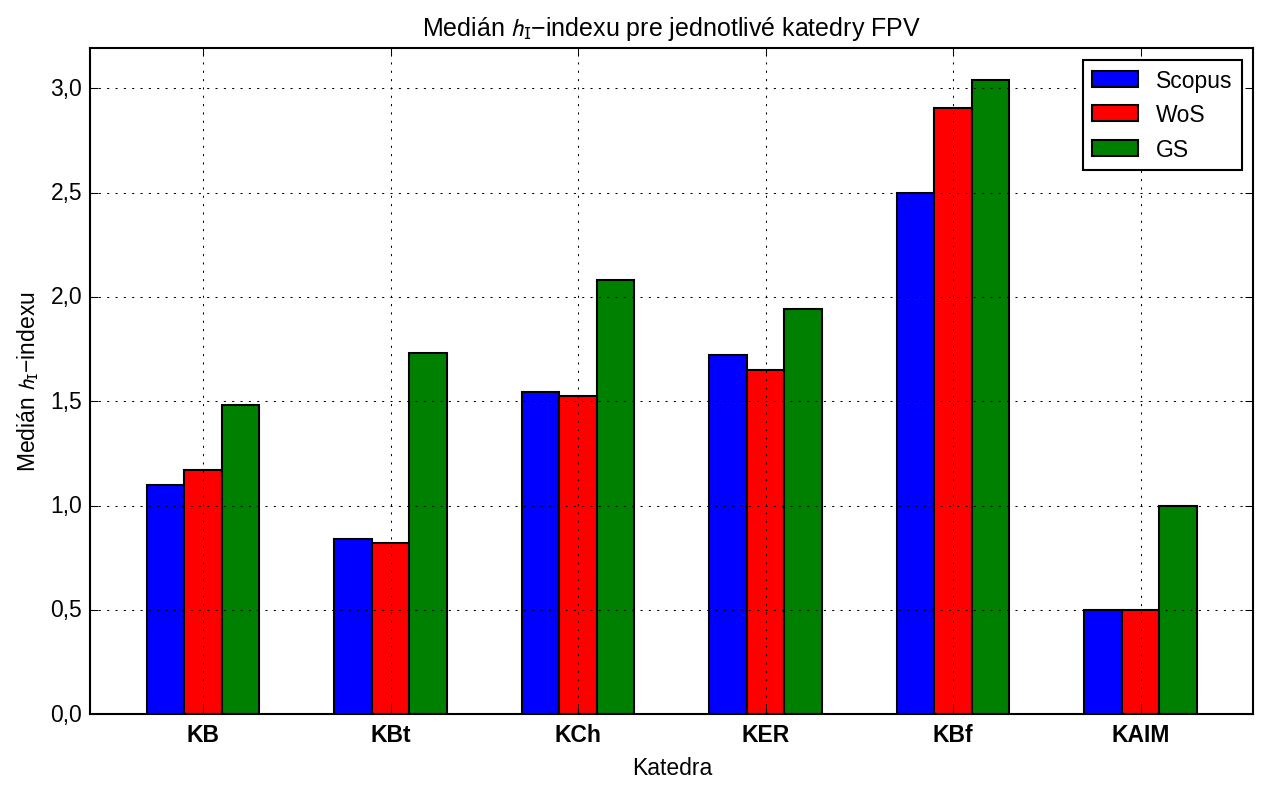
\includegraphics[width=\textwidth]{plot-results-data-hi_index.png}
  \caption{Medián $h_{\mathrm{I}}$-indexu pre jednotlivé katedry FPV UCM v~Trnave}
  \label{fig:hi-index.plot}
\end{figure}

\begin{figure}
  \centering
  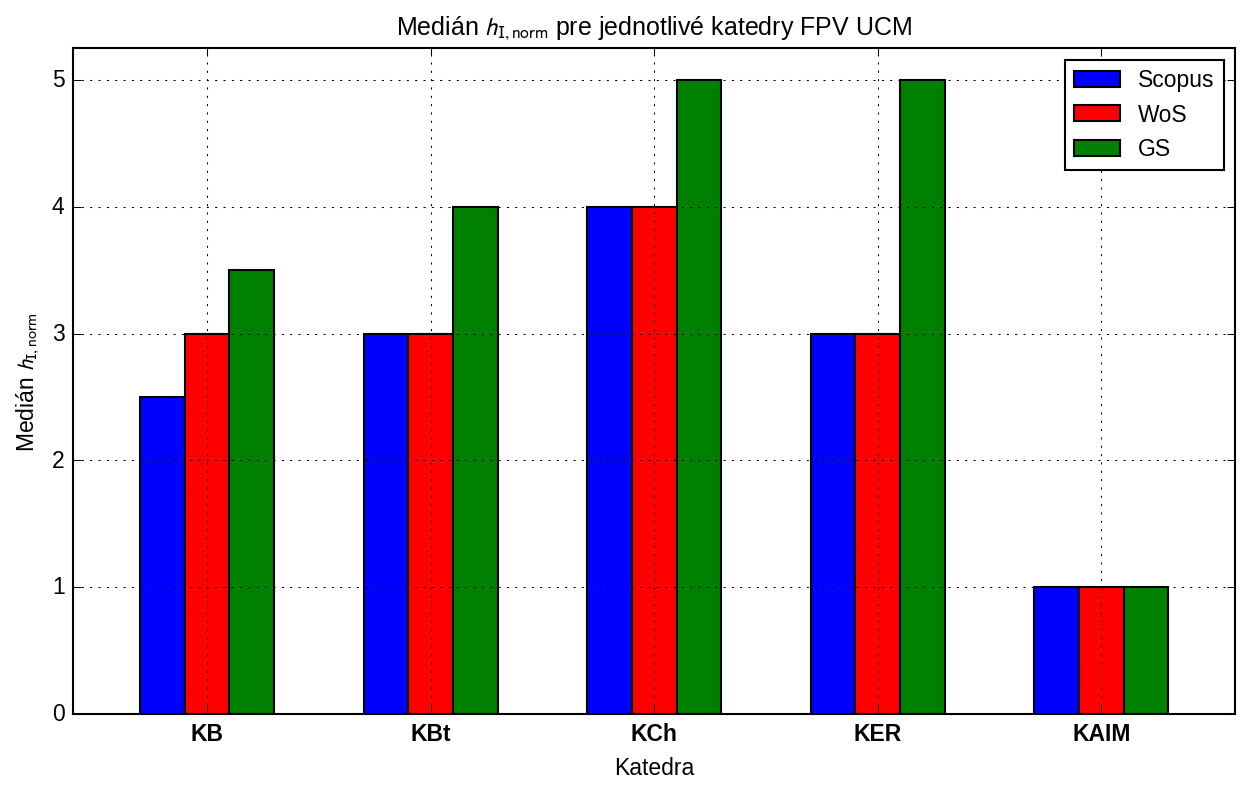
\includegraphics[width=\textwidth]{plot-results-data-hi_norm.png}
  \caption{Medián $h_{\mathrm{I,norm}}$ pre jednotlivé katedry FPV UCM v~Trnave}
  \label{fig:hinorm.plot}
\end{figure}

\begin{table}
  \centering\small
  \caption[Hodnotenie FPV\,--\,AWCR a $AW$-index]%
  {Scientometrické hodnotenie katedier FPV UCM v~Trnave\,--\,AWCR a $AW$-index.}
  \label{tab:5-staff.results}
  \begin{tabularx}{\textwidth}{Xlcccc@{\hspace{3ex}}cccc}
    \toprule\noalign{\vspace{.3ex}}
    & & \multicolumn{4}{c}{AWCR}         & \multicolumn{4}{c}{$AW$-index}  \\
    \cmidrule{3-6}\cmidrule{7-10}
    Katedra & Cit. register & $\bar{x}$ & $\sigma$ & $\tilde{x}$ & MAD & $\bar{x}$ & $\sigma$ & $\tilde{x}$ & MAD \\[0.3ex]
    \midrule\noalign{\vspace{.5ex}}
    KB   & Scopus & 37,50  & 66,36  & 20,21  & 15,31  & 4,64  & 4,15 & 4,46  & 2,25 \\
         & WoS    & 38,77  & 66,64  & 21,65  & 16,82  & 4,83  & 4,09 & 4,65  & 2,45 \\
         & GS     & 23,88  & 91,79  & 22,06  & 15,15  & 24,88 & 4,70 & 4,69  & 1,69 \\[3ex]
    KBt  & Scopus & 59,31  & 121,61 & 24,57  & 9,57   & 5,93  & 5,15 & 4,96  & 1,09 \\
         & WoS    & 33,76  & 54,44  & 19,41  & 9,83   & 4,71  & 3,57 & 4,41  & 1,32 \\
         & GS     & 84,97  & 153,60 & 37,05  & 17,60  & 7,48  & 5,65 & 6,09  & 1,30 \\[3ex]
    KCh  & Scopus & 122,65 & 217,78 & 40,94  & 38,87  & 8,34  & 7,49 & 6,37  & 2,78 \\
         & WoS    & 120,48 & 207,33 & 44,28  & 39,76  & 8,33  & 7,36 & 6,61  & 3,36 \\
         & GS     & 157,82 & 272,44 & 53,79  & 47,38  & 9,56  & 8,39 & 7,29  & 4,40 \\[3ex]
    KER  & Scopus & 45,53  & 28,61  & 58,01  & 12,18  & 6,24  & 2,78 & 7,62  & 0,76 \\
         & WoS    & 40,24  & 26,21  & 46,23  & 15,52  & 5,82  & 2,73 & 6,80  & 1,06 \\
         & GS     & 74,13  & 45,04  & 86,72  & 19,96  & 8,04  & 3,33 & 9,31  & 1,02 \\[3ex]
    KBf  & Scopus & 85,87  & 79,65  & 88,52  & 76,25  & 7,71  & 5,76 & 9,41  & 3,86 \\
         & WoS    & 104,22 & 92,18  & 101,11 & 67,94  & 8,61  & 6,33 & 9,90  & 3,26 \\
         & GS     & 129,18 & 125,84 & 116,20 & 115,44 & 9,50  & 6,98 & 10,78 & 5,81 \\[3ex]
    KAIM & Scopus & 9,17   & 15,03  & 1,50   & 1,50   & 2,10  & 2,28 & 1,22  & 0,94 \\
         & WoS    & 10,07  & 21,56  & 0,25   & 0,25   & 1,73  & 2,77 & 0,50  & 0,50 \\
         & GS     & 18,00  & 28,49  & 3,25   & 3,25   & 3,09  & 3,01 & 1,80  & 1,80 \\[3ex]
    KOJP & Scopus & --     & --     & --     & --     & --    & --   & --    & --   \\
         & WoS    & --     & --     & --     & --     & --    & --   & --    & --   \\
         & GS     & 0,67   & 0,47   & 0,17   & 0,50   & 0,79  & 0,30 & 0,29  & 0,50 \\[0.5ex]
    \bottomrule
  \end{tabularx}
\end{table}

\begin{figure}
  \centering
  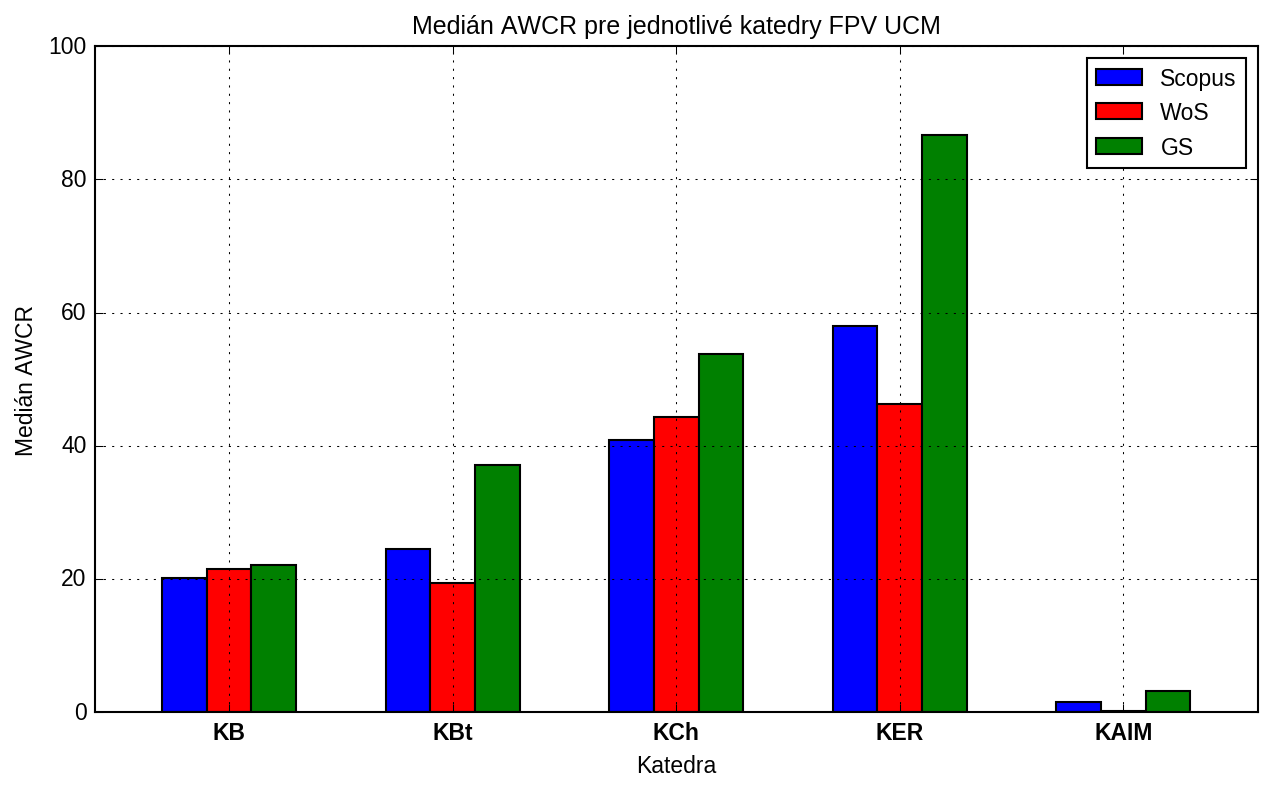
\includegraphics[width=\textwidth]{plot-results-data-awcr.png}
  \caption{Medián AWCR pre jednotlivé katedry FPV UCM v~Trnave}
  \label{fig:awcr.plot}
\end{figure}

\begin{figure}
  \centering
  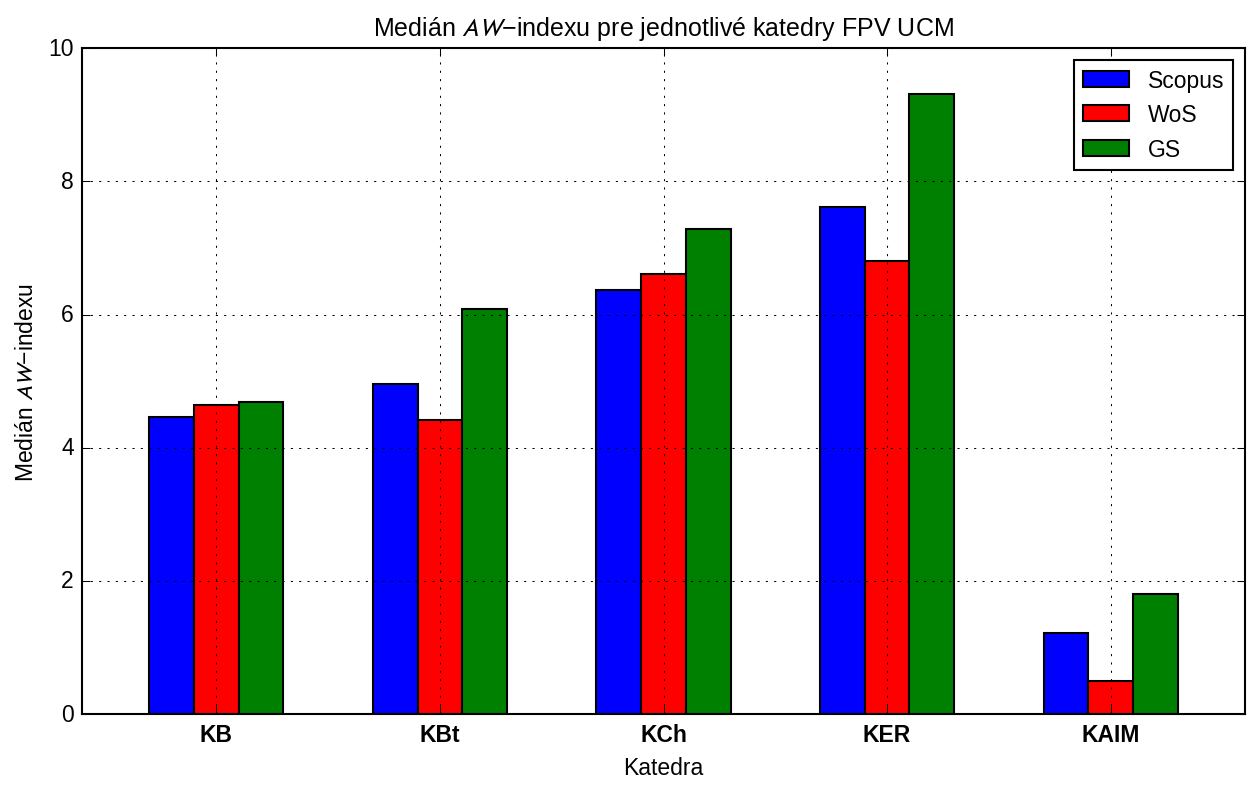
\includegraphics[width=\textwidth]{plot-results-data-aw_index.png}
  \caption{Medián $AW$-indexu pre jednotlivé katedry FPV UCM v~Trnave}
  \label{fig:aw-index.plot}
\end{figure}

\begin{table}
  \centering\small
  \caption[Hodnotenie FPV\,--\,$h^{\mathrm{c}}$-index a $h_{\mathrm{m}}$-index]%
  {Scientometrické hodnotenie katedier FPV UCM v~Trnave\,--\,$h^{\mathrm{c}}$-index a $h_{\mathrm{m}}$-index.}
  \label{tab:6-staff.results}
  \begin{tabularx}{\textwidth}{XXcccc@{\hspace{3ex}}cccc}
    \toprule\noalign{\vspace{.3ex}}
    & & \multicolumn{4}{c}{$h^{\mathrm{c}}$-index} & \multicolumn{4}{c}{$h_{\mathrm{m}}$-index} \\
    \cmidrule{3-6}\cmidrule{7-10}
    Katedra & Cit. register& $\bar{x}$ & $\sigma$ & $\tilde{x}$ & MAD  & $\bar{x}$ & $\sigma$ & $\tilde{x}$ & MAD \\[0.3ex]
    \midrule\noalign{\vspace{.5ex}}
    KB   & Scopus & 5,14  & 4,42 & 4,50  & 2,00 & 3,81  & 5,07 & 1,75 & 1,75 \\
         & WoS    & 5,46  & 4,56 & 5,00  & 2,00 & 4,04  & 5,23 & 2,88 & 1,68 \\
         & GS     & 20,88 & 5,15 & 6,00  & 2,00 & 27,88 & 5,60 & 2,34 & 1,99 \\[3ex]
    KBt  & Scopus & 5,64  & 3,50 & 5,00  & 1,00 & 3,34  & 3,88 & 1,90 & 0,90 \\
         & WoS    & 4,55  & 3,21 & 4,00  & 1,00 & 2,92  & 3,52 & 1,98 & 0,99 \\
         & GS     & 7,18  & 3,74 & 6,00  & 1,00 & 4,66  & 4,58 & 3,33 & 1,30 \\[3ex]
    KCh  & Scopus & 7,94  & 7,68 & 6,00  & 3,00 & 5,03  & 4,81 & 3,17 & 2,22 \\
         & WoS    & 7,94  & 7,39 & 6,50  & 3,50 & 5,40  & 5,16 & 3,06 & 2,26 \\
         & GS     & 9,44  & 8,49 & 8,00  & 4,00 & 6,26  & 6,22 & 3,59 & 2,45 \\[3ex]
    KER  & Scopus & 7,00  & 2,83 & 8,00  & 1,00 & 3,57  & 2,47 & 3,87 & 1,41 \\
         & WoS    & 6,14  & 2,34 & 7,00  & 1,00 & 3,31  & 2,26 & 3,70 & 0,98 \\
         & GS     & 8,00  & 3,00 & 9,00  & 1,00 & 4,44  & 2,44 & 4,41 & 2,49 \\[3ex]
    KBf  & Scopus & 8,00  & 6,08 & 11,00 & 2,00 & 5,62  & 5,01 & 6,79 & 3,86 \\
         & WoS    & 9,00  & 7,07 & 9,50  & 4,50 & 6,45  & 5,00 & 6,91 & 3,11 \\
         & GS     & 9,80  & 7,60 & 11,00 & 7,00 & 6,49  & 5,32 & 7,09 & 5,01 \\[3ex]
    KAIM & Scopus & 2,09  & 1,97 & 2,00  & 2,00 & 2,56  & 4,01 & 0,83 & 0,67 \\
         & WoS    & 1,46  & 2,15 & 1,00  & 1,00 & 2,45  & 4,44 & 0,50 & 0,50 \\
         & GS     & 2,87  & 2,75 & 2,00  & 2,00 & 2,93  & 4,40 & 1,25 & 1,25 \\[3ex]
    KOJP & Scopus & --    & --   & --    & --   & --    & --   & --   & --   \\
         & WoS    & --    & --   & --    & --   & --    & --   & --   & --   \\
         & GS     & 1,00  & 0,00 & 0,50  & 0,50 & 0,67  & 0,47 & 0,50 & 0,34 \\[0.5ex]
    \bottomrule
  \end{tabularx}
\end{table}

\begin{figure}
  \centering
  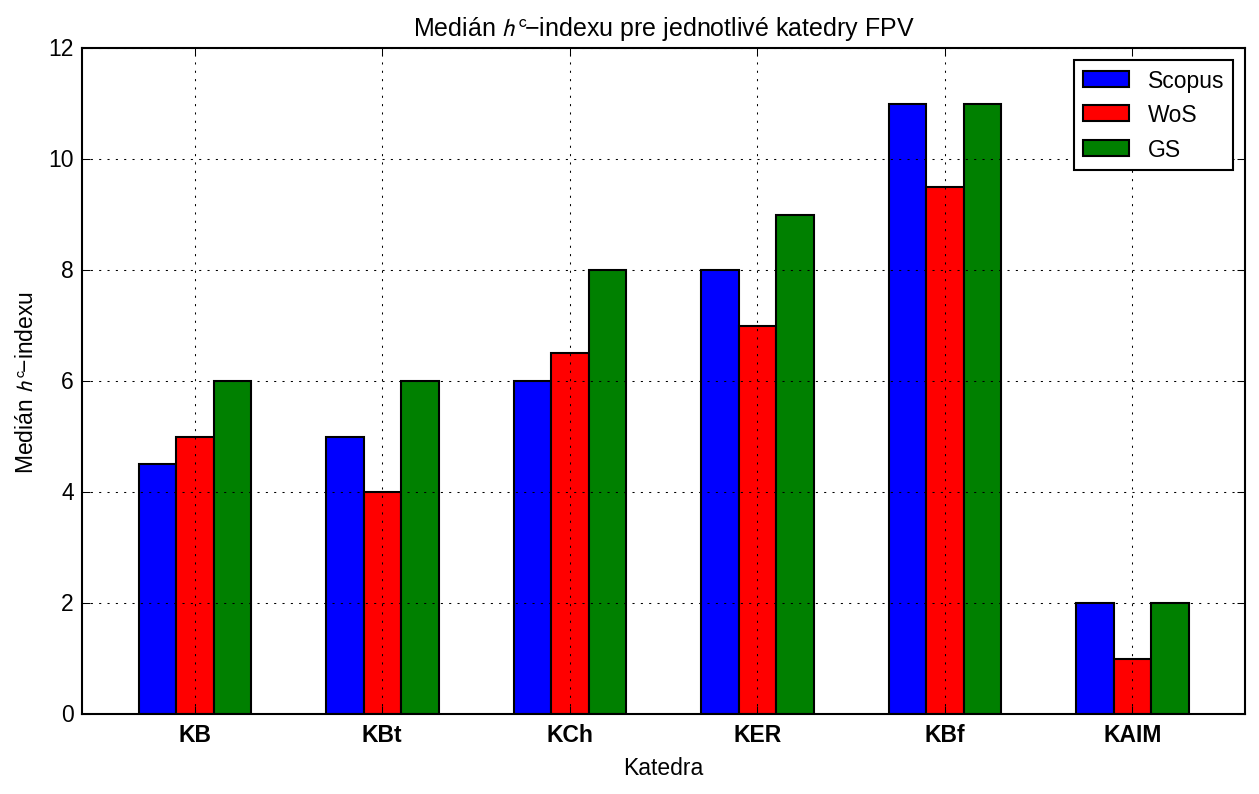
\includegraphics[width=\textwidth]{plot-results-data-hc_index.png}
  \caption{Medián $h^\mathrm{c}$-indexu pre jednotlivé katedry FPV UCM v~Trnave}
  \label{fig:hc-index.plot}
\end{figure}

\begin{figure}
  \centering
  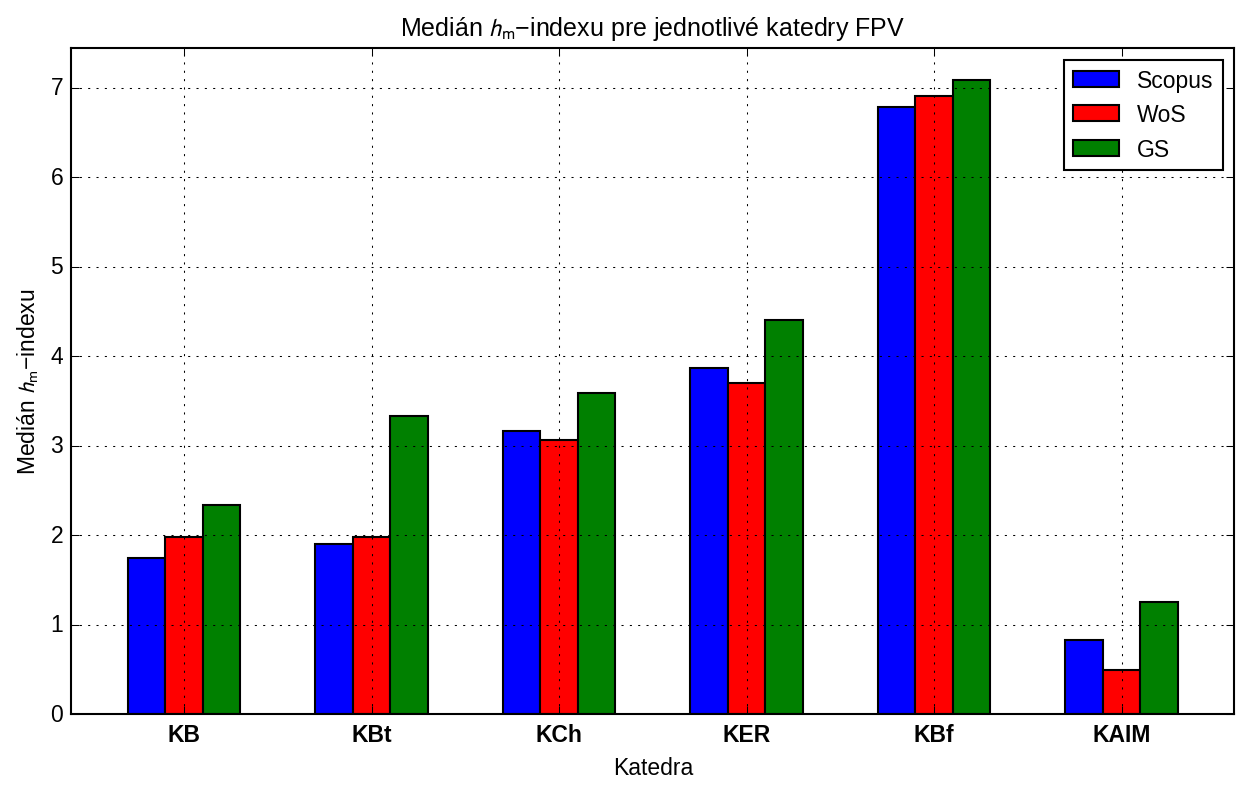
\includegraphics[width=\textwidth]{plot-results-data-hm_index.png}
  \caption{Medián $h_\mathrm{m}$-indexu pre jednotlivé katedry FPV UCM v~Trnave}
  \label{fig:hm-index.plot}
\end{figure}

\begin{figure}
  \centering
  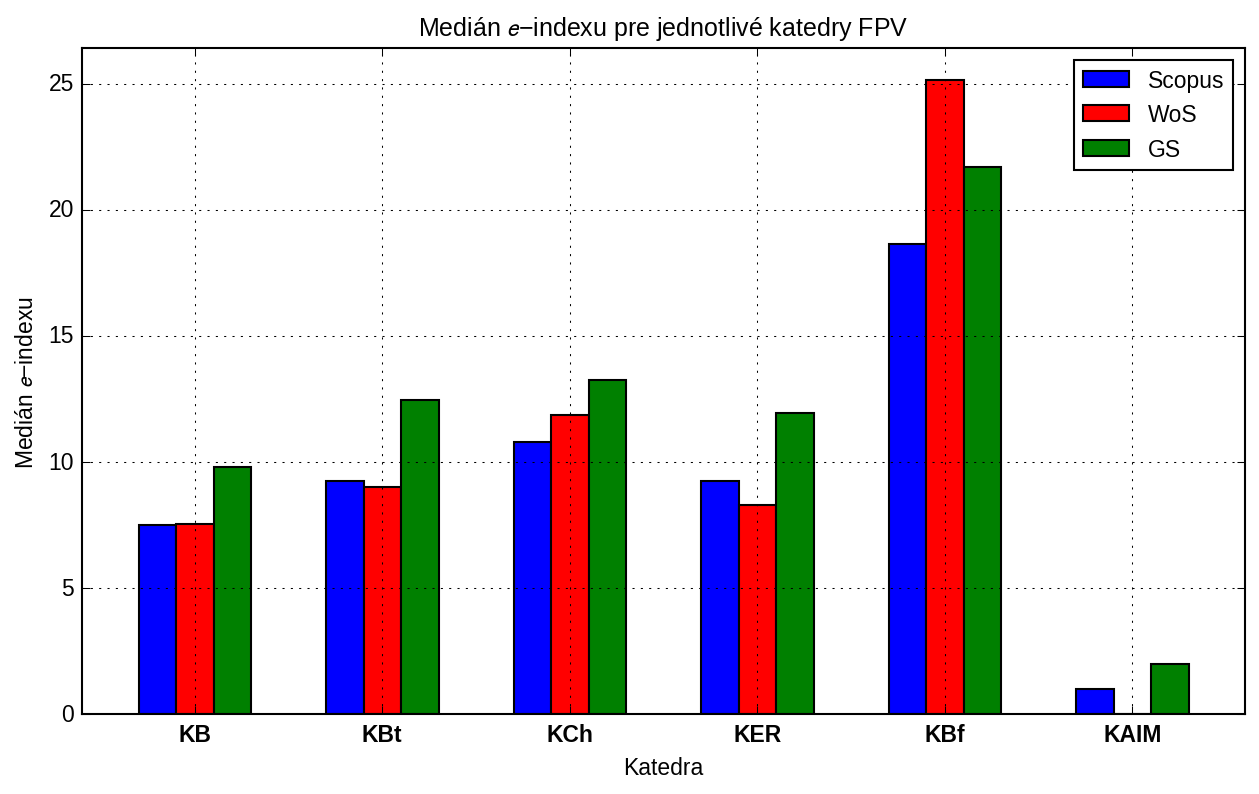
\includegraphics[width=\textwidth]{plot-results-data-e_index.png}
  \caption{Medián $e$-indexu pre jednotlivé katedry FPV UCM v~Trnave}
  \label{fig:e-index.plot}
\end{figure}


%%% Local Variables:
%%% TeX-master: "diplomovka"
%%% End:
